%BitTorrent
\section{BitTorrent}
BitTorrent \citep{bittorrent:bep03} is a peer-to-peer protocol for file sharing designed by Bram Cohen in 2001.
The protocol is responsible for around 30 percent of the data uploaded to the internet.
The traditional way to ose the bittorrent protocol is to use a BitTorrent desktop client. That is a computer program that implements the BitTorrent protocol.
The .torrent files comes with a metadata file that includes a trackerlist. The bittorrent tracker is a server that contains information about what peers are interested in a given torrent. The tracker can connect a peer to other peers with the same torrent so the first peer can download and upload torrent data from and to those peers.

\subsection{File sharing}
Torrents is a very popular and easy method to share large files, because every user providing bandwidth i.e. the seeding of the torrents.
The payload of the server that initially shared the file does not have to be big, because the user will share the file with other users instead of overloading the server.
%tracker hash forbinde folk 

\section{HTML5}
Html 5 is the latest markup language for writing web applications is was relaesed in 2014. Some of the new tags introduced is video and audio tags wich makes it possiple to play video and audio in the player build into html5.

Html5 also implements local storage. This makes it possible to store content locally in the browsers rather than use cookies, to store the data.
The storage limit it larger than when using cookies (at least 5mb) and the data is stored locally so it does not need to be sent to a server.

\section{Popular music streamers}
The are many music-streamers already reseased and we will let us get inspired by some of the most popular and give a walktrough of them below.

\subsection{Spotify}
Spotify is the most popular online music streamer. The program was released in 2006 and was developed in Sweeden Stockholm by Daniel Ek and Martin Lorentzon. Now their main office is placed in Luxemborg and they have devisions in Stockholm and Göteborg. Their buisness model is that customers can listen to music in exchange for listening to commercials between tracks, or they can pay a monthly fee to be premium members.
The music is placed on servers controlled by spotify in contrast to the peer-to-peer music streamer we will develop.
\begin{figure}[h]
  \centering
    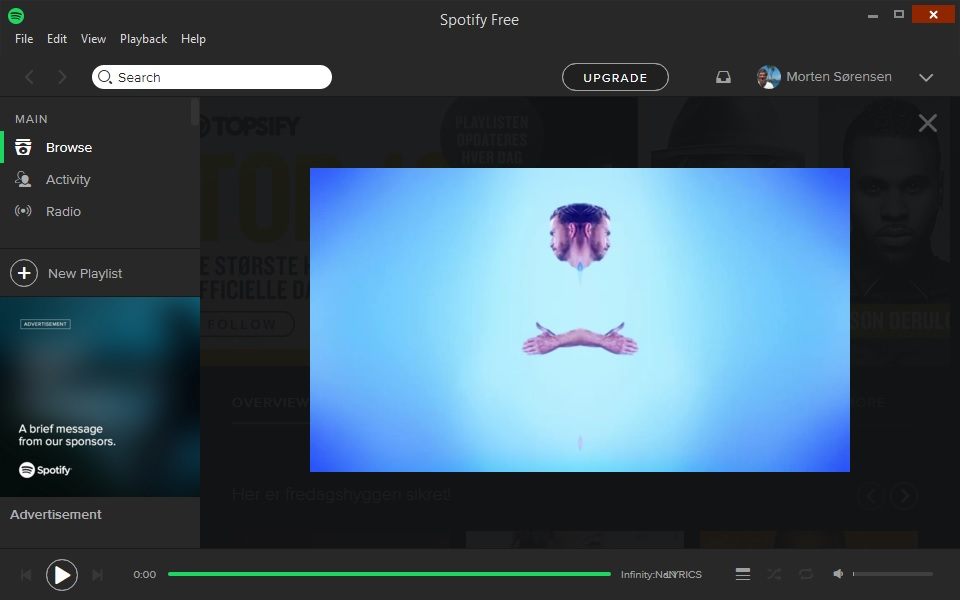
\includegraphics[width=0.9\textwidth]{gfx/Spotify_desktop.jpg}
  \caption{A picture of the GUI in the Spotify desktop application}
  \label{fig:spotify}
\end{figure}
As seen in \ref{fig:spotify} the music player is placed in the buttom of the application, there is a menu at the left of the screen where your personal playlists can be accessed, and where it is possible to browse for new music and listen to a radio channel.
Spotify now have over 75 mission active users, both from Europe, America and Asia. Spotify both have clients for desktops and mobiles.

\subsection{Napster}
Napster was when it was released in 1999 a peer-to-peer file sharing service that focussed on audio files. Napster was co-founded by Shawn Fanning, John Fanning, and Sean Parker The Napster site was only operational untill 2001 because it was sued by Metallica for sharing music illigally. It was then brought down by court order. Metallica learned that their song "I dissapear" was avaiable on Napster before it was released witch also led to it be played on radios. Napster peaked at 25 million users in january 2001 On March 13, 2000 Metallica filed a lawsuit against Napster. Many  In addition to the Napster weppage, a desktop client was developed both to windows and later to MAC OS.
Napster had to pay 36\$ in royalties to various music companies and had to declare itselves bankrupt. Roxio bought the assets of Napster to relaunch it as a online music store, where users had to pay money for each track. In may 2006 Roxio launched a free verion of Napster where users where able to stream full length tracks, where the service was powered by adds. They had the limit that each song could only be streamed 3 times each by every user, but they had 8million songs to choose from.
The free Napster service was discontinued in March 2010, because Napster was sold to Best Buy in January 2010.
Rapsody (another streaming and download service) bought Napster in 2011 and transformed it into a subscription based streaming client for desktop or phones.

\subsection{Popcorn-Time}
Popcorn-time is a multi-platform bittorrent client for streaming videos. The popcorn-time interface is much simillar to that of Netflix. It presents the user with thumbnail immages of the movies and when the user selects a picture the movie is then downloaded with the bittorrent protocol, and played in the build-in player.
 When a download starts the movie is also seeded to other peers in the network. The seeding continues until the content i deleated with usually happens when the application closes.
 In 2014 developers made popcorn-time available on android, and support for Chromecast and Apple TV.

\subsection{Netflix}
Netflix is the largest streaming company. As seen in \citep{netflix} they were looking into the possibilities of using webtorrent in their company. At the time of the article Netflix had a job application for a peer-to-peer senior developer. Netflix is not using any peer-to-peer protocol today so the project was not a huge success.

\section{Browser versus desktop}
The above mentioned systems are either implemented via. a web-browser +
centralized backend server, or by means of a desktop application.

To ease usability we've decided that our application must run within the
context of the web-browser. I.e. that users will not have to install a desktop
application first. This has several implications, amongst others;
\begin{itemize}
\item Limited access to hardware
\item Limited connection layer technologies
    \begin{itemize}
        \item HTTP
        \item WebSockets
        \item WebRTC
    \end{itemize}
\item Limited access to persistent storage
    \begin{itemize}
        \item LocalStorage
        \item IndexedDB
        \item WebSQL
    \end{itemize}
\end{itemize}
We are aware of the fact, that these limitations will make it harder for us to
prove our hypothesis, but we believe that the proof will be stronger and more
convincing given the limitations of the web-browser context.

\subsection{Browserify}
Browserify is a tool, which bundles up multiple javascript files into a single
file, it does so by intelligently parsing files, and handling include
statements, this enables us to write code with utilizes \verb|node.js|'s require
include within our code, and additionally enables us to utilize libraries from
the node package manager (\verb|npm|), a workthrough of the most significant 
libraries we've utilized can be found in section~\ref{sec:libraries}.

Additionally browserify handles multiple target arcitectures; I.e. the browser,
and the node.js desktop environment. We originally envisioned creating both a 
web-interface and a more technical desktop client, but due to time constaints,
we've limited ourselves to the desktop client.

\section{WebSocket}
% TODO: Was it html5?
WebSockets are a transport layer technology introduced in HTML5, it enables BSD
socket-like data transfers between the browser and a web-socket enabled backend
server. That is; a single open bi-directional connection, over which multiple
messages may be transmitted.

% TODO: How does it work?
A WebSocket connection is intialized by a HTTP request, bla bla bla.

% TODO: more


\section{Web-RTC}
WebRTC is a javascript API drafted by W3C that establishes support for browser-to-browser connections,
instead of traditional client-server connections like WebSockets, AJAX and Server Sent Events.
These client-server networks suffer from high latency, and do not allow browsers to act as a server,
as browsers cannot listen for WebSocket connections.

It was originally intended to support real-time-communication (RTC) 
and allow browsers to easily establish audio and video teleconferencing and telecommunications
using its three primary APIs: MediaStream, RTCPeerConnection and RTCDataConnection.
The RTCDataConnection part of the API is particularely interesting
as it allows arbitrary application data to be sent betweeen browsers,
allowing a myriad of peer-to-peer techniques to be implemented as WebRTC code for browsers.

Before WebRTC, establishing direct peer-to-peer connections in the browser required
additional plugins in the browser such as Flash or Java, which would then download the necessary networking code
from a server and execute it locally,
these plugins did not come with most browsers,
which means many users did not have them available.
\newline

% TODO: write about peerconnection requiring central server to establish connection
\label{webrtc-connection-server}
When using WebRTC, we must first notify the remote peer of our intention
to open a peer-to-peer connection, so it can start listening for incoming packet,
we also have to establish the necessary routing paths to each other peer on both sides,
and relay this information,
and finally establish the intended parameters: protocols, encoding used, and so on.

For the purposes of notifying the remote peer, a signaling service is necessary,
this means having a centralized server that the browser contacts and asks to have a connection created.
The signaling service does not need to be involved after the connection has been established,
it can free up its resources to focus on signaling for new peers, 
while the already established connections can continue regardless of whether the signalling service has quit.

%% FRAMEWORKS
%
TODO

